              
                %%%%%%%%%%%%%%%%%%%%%%%%%%%%%%%%%%%%%%%%%%%%%%%%%%%%%%%%%%%%%%%%%%%%%%
% LaTeX Example: Project Report
%
% Source: http://www.howtotex.com
%
% Feel free to distribute this example, but please keep the referral
% to howtotex.com
% Date: March 2011 
% 
%%%%%%%%%%%%%%%%%%%%%%%%%%%%%%%%%%%%%%%%%%%%%%%%%%%%%%%%%%%%%%%%%%%%%%
% How to use writeLaTeX: 
%
% You edit the source code here on the left, and the preview on the
% right shows you the result within a few seconds.
%
% Bookmark this page and share the URL with your co-authors. They can
% edit at the same time!
%
% You can upload figures, bibliographies, custom classes and
% styles using the files menu.
%
% If you're new to LaTeX, the wikibook is a great place to start:
% http://en.wikibooks.org/wiki/LaTeX
%
%%%%%%%%%%%%%%%%%%%%%%%%%%%%%%%%%%%%%%%%%%%%%%%%%%%%%%%%%%%%%%%%%%%%%%
% Edit the title below to update the display in My Documents
%\title{Project Report}
%
%%% Preamble
\documentclass[paper=letter, fontsize=11pt]{scrartcl}
\usepackage{url}
\usepackage{color}
\usepackage{fourier}
\usepackage{listings}
\usepackage[T1]{fontenc}
\usepackage[spanish]{babel}
\selectlanguage{spanish}
\usepackage{hyperref}
\usepackage[pdftex]{graphicx}
\usepackage[margin=2.5cm]{geometry}
\usepackage{amsmath,amsfonts,amsthm} % Math packages
                                       % English language/hyphenation
\usepackage[protrusion=true,expansion=true]{microtype}  

%%% Maketitle metadata
\newcommand{\horrule}[1]{\rule{\linewidth}{#1}}     % Horizontal rule

\title{
        %\vspace{-1in}  
        \usefont{OT1}{bch}{b}{n}
        \normalfont \normalsize \textsc{Universidad de los Andes, Departamento de F\'isica \\
        F\'isica at\'omica} \\ [25pt]
        \horrule{0.5pt} \\[0.4cm]
        \huge Oscilador arm\'onico \\
        \horrule{2pt} \\[0.5cm]
}
\author{
        \normalfont                                 \normalsize
        Juan Barbosa, 201325901\\[-3pt]      \normalsize
        Febrero 23, 2017
}
\date{}

\lstset{keywordstyle=\color{blue}, basicstyle=\scriptsize, frame=single, language=Python}

%%% Begin document
\begin{document}
\maketitle

\[
\boxed{-\dfrac{\hbar^2}{2m}\nabla^2\Psi(x) + V(x)\Psi(x) = E\Psi(x)}
\]

Para un oscilador arm\'onico la energ\'ia potencial se escribe:
\begin{equation}
	V(x) = \dfrac{1}{2}kx^2 = \dfrac{1}{2}m\omega^2x^2
\end{equation}

La ecuaci\'on de Schr\"odinger se escribe de la forma:
\begin{equation}
	\dfrac{d^2}{dx^2}\Psi(x) = \ddot{\Psi}(x) =  \dfrac{2m}{\hbar^2}\left(\dfrac{1}{2}m\omega^2x^2-E\right)\Psi(x)
\end{equation}

La soluci\'on a la ecuaci\'on anterior debe cumplir que para $x = \pm\infty$, $\Psi(x) = 0$. Las soluciones anal\'iticas usan los polinomios de Hermite.
\begin{equation}
	\Psi_n(x) = \dfrac{1}{\sqrt{2^nn!}}\left(\dfrac{m\omega}{\pi\hbar}\right)^{1/4}e^{-\frac{m\omega x^2}{2\hbar}}H_n\left(\sqrt{\dfrac{m\omega}{\hbar}x}\right)
	\qquad \text{donde} \qquad	H_n(x) = (-1)^ne^{x^2}\dfrac{d^n}{dx^n}e^{-x^2}
\end{equation}

Usando el m\'etodo de Euler para resolver num\'ericamente se obtiene:
\begin{equation}
	\begin{matrix}
	\dot{\Psi}_n = \dot{\Psi}_{n-1} + \ddot{\Psi}_{n-1}\Delta x \\
	\Psi_n = \Psi_{n-1} + \dot{\Psi}_n\Delta x
	\end{matrix}
\end{equation}

El sistema de ecuaciones diferenciales es resuelto en C usando $N = 100000$ puntos, $dx = 0.0001$, para $\omega = 0.4, 0.6, 0.8, 1.0$. Las unidades usadas son arbitrarias tales que $\hbar^2 = m = 1$. Posteriormente se usa un algoritmo en Python para graficar las soluciones.

\newpage
\lstinputlisting[language=C]{seeker.c}
\lstinputlisting{plotter.py}
\newpage
\begin{figure}[ht]
	\centering
	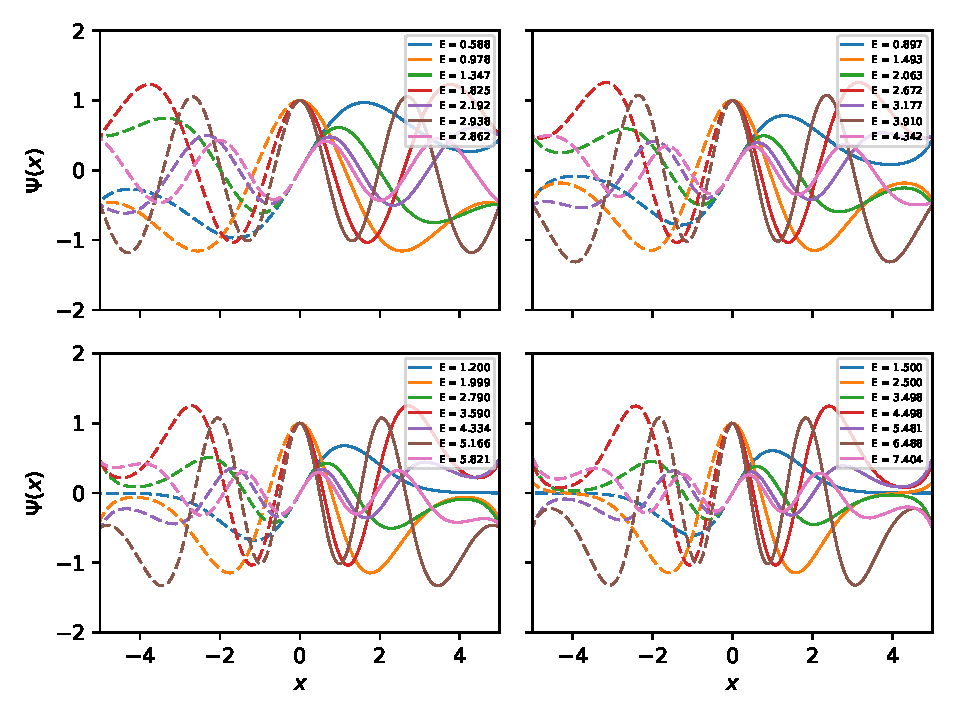
\includegraphics[width=0.8\linewidth]{plot.pdf}
	\caption{Funciones de onda con mejores comportamientos asist\'oticos.}
	\label{fig:waves}
\end{figure}
\begin{figure}[h!]
	\centering
	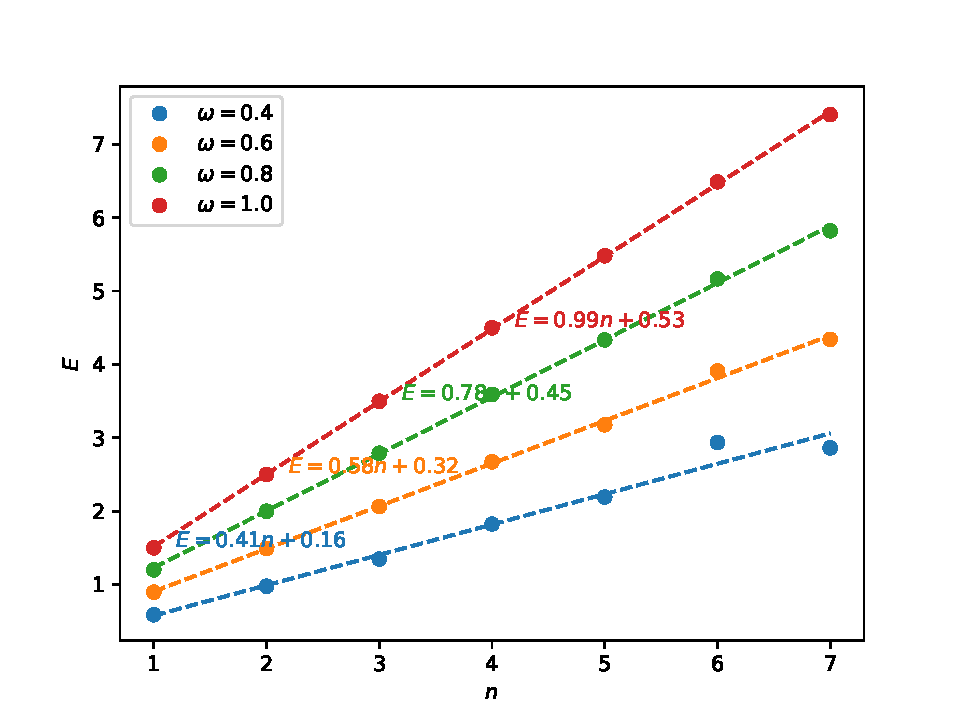
\includegraphics[width=0.5\linewidth]{energies.pdf}
	\caption{Energ\'ia en funci\'on de $n$, para distintos valores de $\omega$.}
	\label{fig:energies}
\end{figure}

En la \autoref{fig:waves} se muestra las funciones de onda para las cuales se considera convergencia en el algoritmo en C, las funciones son simuladas de $x=0$ hasta $x=10$, la l\'inea punteada corresponde por simetr\'ia con $x<0$. En la \autoref{fig:energies} se muestran los valores que adquiere la energ\'ia para distintos valores de $n$ y $\omega$. Al observar las regresiones lineales se puede establecer la siguiente relaci\'on.
\begin{equation}
	E_{n\omega_i} \propto \omega_in \qquad \implies \qquad E_{n\omega} \propto \omega n
\end{equation}
\end{document}
              